\documentclass[10pt,conference,compsocconf]{IEEEtran}

\usepackage{hyperref}
\usepackage{graphicx}	% For figure environment
\usepackage{authblk}
\usepackage{tabularx}
\usepackage{float}

\title{Project 2 on Machine Learning\\Text classification\\Team Yoor}

\author[1]{Sergei Volodin}
\author[1]{Baran Nama}
\author[1]{Omar Mehio}
\affil[1]{EPFL}
\affil[ ]{\textit {\{sergei.volodin,baran.nama,omar.mehio\}@epfl.ch}}

\begin{document}

\maketitle

\begin{abstract}
A classification dataset consisting of Tweets is being studied. First, the data is thoroughly explored using visual aids. Several basic Natural Language Processing methods are applied. Results are evaluated using cross-validation. Model overview is given and the best model is chosen.
\end{abstract}

\section{Introduction}
This paper investigates into improving the quality of sentiment analysis on Tweets dataset \cite{kaggle}.
It consists of $N_1=N_2=1250000$ positive/negative tweets, each of them representing a message in English and numerical alphabet $\Sigma$ with no longer than 140 characters.
This way, each of $N=N_1+N_2=2500000$ tweets is assigned to one of the classes $\mathcal{C}=\{\mbox{:(},\,\mbox{:)}\}$.
The task is to minimize the classification error.
In other words, if $\mathcal{D}=\{(x_n, y_n)\}_{n=1}^N$ is the dataset with tweets $x_i\in\Sigma^*$ being messages and $y_n\in \mathcal{C}$ being class labels, the goal is to train a classifier $f\colon\, \Sigma^*\to\mathcal{C}$ which minimizes the loss function $l(y,\hat{y})=[y\neq \hat{y}]$.

The task of sentiment analysis of tweets was thoroughly studied \cite{sota1, sota2, sota3, sota4}. These solutions usually give accuracy around 80\%.
Several techniques were applied, mostly consisting of two steps.
First, the words are converted to dense vectors using Glove, word2vec, cbow or skip-gram models.
After that, the resulting word vectors are used to construct features for the whole tweet.
At the end, the vector is feeded into a classifier, such as SVM or Logistic Regression.
Two latter steps might be replaces with a neural network accepting variable-length input such as RNN or CNN.
Moreover, the embeddings themselves might be trained using backpropagation while training the classifier.

Claim: it is possible to find a model which fits the data better than the current state-of-the-art using expert knowledge on the Tweets dataset.

Next sections describe in details our approaches and compare them to various baselines.
\section{Models and Methods}
\subsection{Data cleaning}
\newcolumntype{L}[1]{>{\hsize=#1\hsize\raggedright\arraybackslash}X}%
\newcolumntype{R}[1]{>{\hsize=#1\hsize\raggedleft\arraybackslash}X}%
\newcolumntype{C}[1]{>{\hsize=#1\hsize\centering\arraybackslash}X}%

\begin{table*}[htbp]
	\centering
	\small
	\begin{tabularx}{\textwidth}{| L{0.1} | L{0.05} | L{0.7} | L{0.2} | }
		\hline
		Class&Row&Message&Comment\\
		\hline
		:( & 171 & {\tt <user> 5k i could cry i'm so unfit !} & User tag \\\hline
		:( & 99804 & {\tt if i feel like this tomorrow i'm going to the er } & Contraction, missed comma\\\hline
		:) & 524 & {\tt its the weekend ! ! <user> s coming home anddd <user> s baby shower , exciteddd } & Letter repetitions\\\hline
		:) & 99615 & {\tt <user> aren't you just an adorable granny <url> } & URL tag\\\hline
		:) & 443 & {\tt <user> :d :d :d :d :d wish jocelyn had a twitter . \#kudos for her too . } & Hashtag, emoticons \\\hline
		:) & 468 & {\tt retweet if you was born in the 90 ' s ! \#90's babies } & Grammar\\\hline
		:( & 14 & {\tt <user> i'm white . \#aw } & Appear neutral \\\hline
		:( & 99594 & {\tt <user> <user> <user> they're there tonight ! ! ! } & Appear positive \\\hline
	\end{tabularx}
	\caption{Examples of tweets in the small dataset}
	\label{tab:tweet-sexample}
\end{table*}

This paragraph describes the data being studied.
Tweets are short messages no longer than 140 characters long \cite{twitter}.
The table \ref{tab:tweet-sexample} represents a few examples from the small dataset.
Being considered an informal way of communication, tweets often contain misspelled words and letter repetitions, grammatical and other writing mistakes.
Besides plain text with punctuation, tweets also contain hashtags, two types of tags, {\em user} and {\em url}, which are tokens for replaced user mentions and URL links, respectively.
In addition, tweets sometimes contain emoticons.
Despite the fact that objects in the training dataset mostly comply with its classes, some tweets cannot be determined as positive/negative even by a human (appear neutral).
Moreover, some of the tweets are clearly mislabeled in the training data.
Dataset contains repeating tweets.

Representation of tweets was through the occurency matrix, where each row corresponds to a tweet , each column corresponds to a term in the vocabullary and each cell corresponds to the number of times this word occurrs in this tweet. Through preprocessing the aim is to maximise the knowledge that can be extracted from the datasets in order to build this matrix.  Hence th focus was on increasing the occurence of words through correction of misspelled words and stemming techniques.

Usually tweeters repeat a letter in a word to stress on a certain emotion , as an example : "i am soooooo angryyyy".This problem was tackled by two approaches.
The first approach is called stemming.A formal definition of stemming : is the process by which we find the origin of the word. Linguistically any word can be changed to different forms by either adding afixes or prefixes, thus one word can have multiple forms, all corresponding to the same origin.Through stemming, the aim is to minimise the presence of these different forms and replacing them with the original stem. Algorithm
We do this by replacing every repeated letter by two instances of that letter.We check if the word is valid (contained in a dictionary) if it is the case then we found the correct form of the word, otherwise we reccurr on the new word.Our end result is a set of tweets with most of the words having repeated characters replaced by their stems.

\begin{figure}[!htb]
	\centering 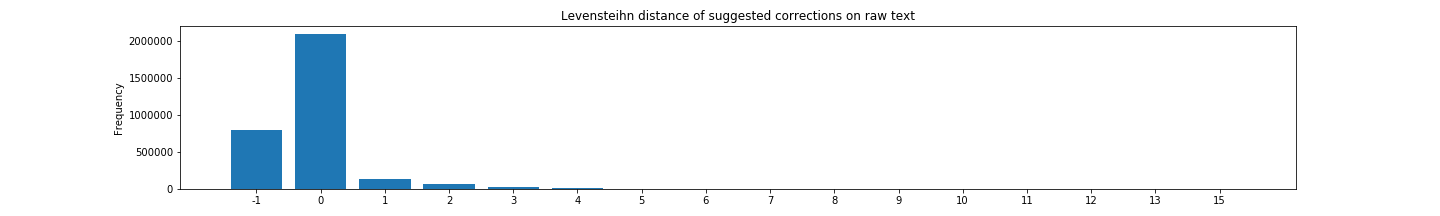
\includegraphics[height=100px,width=100px]{../plots/distributionA.png}
	\caption{Exploratory data analysis using charts}
	\label{fig:data}
\end{figure}

The second approach adopted is misspelling correction. The process goes as follows : a token in the tweet is proposed to an english dictionary, the dictionary responds by either indicating that the word is valid or not. This dictionary provides the most relevant suggestions to correct this word. As a metric to modify a word , the levenshtein distance was use.Levenshtein distance is defined as : "the distance between two strings is the minimal number of insertions, deletions, and substitutions of one character for another that will transform one string into the other". Thus to explore how many misspelled-wrong words are in the dataset , we ploted the distribution in Fig []. All most of the data correction is covered by setting our levensteihn threshold to 4.

\begin{figure}[!htb]
	\centering 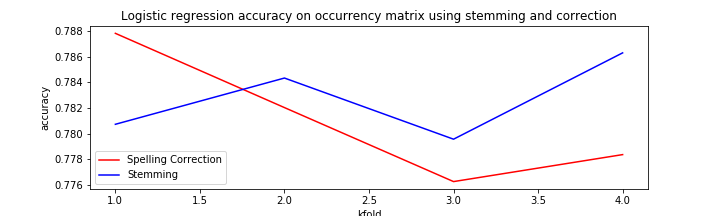
\includegraphics[width=200px]{../plots/raw.png}
	\caption{Exploratory data analysis using charts}
	\label{fig:data}
\end{figure}

The metric used to compare both methods was prediction accuracy of logistic regression. As a first step the combined dataset of both the positive and negative tweets was exposed to stemming and correction. Then for each method a vocabullary of words is constructed. Finally, the occurrence matrix is built from both the tweets and the dictionary. K-fold is used to split the matrix and then logistic regression is run using the occurrence matrix as the data matrix, labels are split into 0 denoting positive sentiment and 1 denoting, a negative sentiment.  As observed in figure x , the spelling correction method is superficial to the stemming method with reaching a maximum of 78.6 % prediction accuraccy.


\begin{figure}[!htb]
	\centering 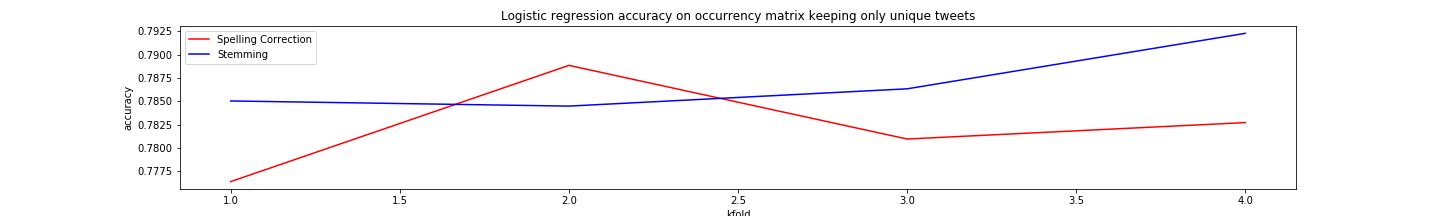
\includegraphics[width=200px]{../plots/redundant.png}
	\caption{Exploratory data analysis using charts}
	\label{fig:data}
\end{figure}

Another property observed in the dataset is the presence of redundant tweets. To view their impact ,repeated instances of a tweet are eliminated and the newly formed unique dataset is exposed to the previous methods. And as observed once again the correction spelling method overpowers the stemming technique. Although with very small improvement in accuracy prediction (78.88%).

\begin{figure}[!htb]
	\centering 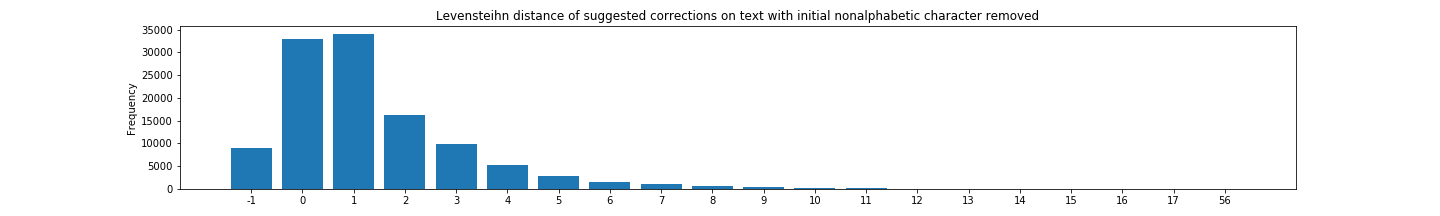
\includegraphics[width=200px]{../plots/distributionB.png}
	\caption{Exploratory data analysis using charts}
	\label{fig:data}
\end{figure}

According to fig ,we can observe that many tokens in our datasets start with non alpahbetic characters. Those tokens were eliminated from the previous experiments as all dictionaries cann't recognize non alphanumeric words. Thus  a new set of tweets was constructed having all tokens that contain characters, but start with a non-alphabetic character to be stripped of that character or characters.AS before, the distribution of levensteihn distances for suggested words was plotted,which results in a more uniform distribution. It is suspected that this is due to the informal language used in hashtags. 
\begin{figure}[!htb]
	\centering 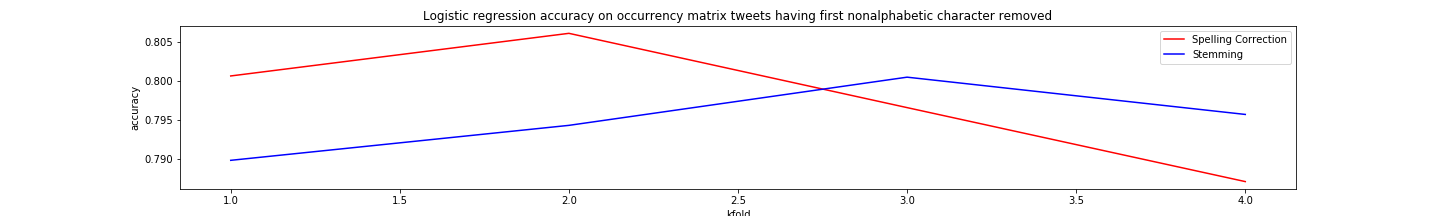
\includegraphics[width=200px]{../plots/filtered_text.png}
	\caption{Exploratory data analysis using charts}
	\label{fig:data}
\end{figure}
The newly constructed dataset is aplied to previous methdods .Eliminating redundant tweets , since as observed this gave us a slight improvement. Then the dataset is exposed it to stemming and misspelling correction. Accuracy prediction then improves to 0.802 , the best score ever reached.

Now with the optimal model having intial nonalphabetic characters removed , redundant tweets eliminated and misspelling correction applied with levensteihn threshold set to 5.The dataset is tackled from a different angle,the effect of the frequency of which one token appears in the document is explored. Thus two approaches are considered : removing most frequent tokens that are common in both datasets and removing nonfrequent words from the vocabullary. The results of the first experiment came as a surpise.As suspected that common words would make it harder for the classifier to distinguish between a positive sentiment tweet and a negative one.A reasoning for that is a due to the limited number of characters provided to users to express themselves and thus most of the tweet gets distributed among tagging other users,using punctuation and stopwords to express feelings.Also eliminating non frequent tokens from our vocabullary has helped improving accuracy , as observed in fig.

\subsection{Prediction models}
A several models were considered.
First, the baseline was the GloVe \cite{glove} model, which is considers training embeddings on the co-occurence matrix.
Unfortunately, the model did train quite slow on the dataset gave meaningless embeddings (closest words for a given word did not correspond to it in meaning).
Therefore, it was not considered.

Secondly, a word count model was considered as a replacement.
Here, a tweet is represented by a high-dimension sparse vector, each item corresponds to a number of occurences of this word in the tweet.
This vector was further classified using several techniques, such as SVM and Neural Network.
This method gave higher accuracy and allowed for tweaking its parameters with relatively small training time (a Google Cloud instance with 8 CPU was used)
\vspace{5mm} %5mm vertical space
\subsubsection{Convolutional neural networks (CNN)}


One of the method that we tried for tweet classification is convolutional neural networks. Convolutional neural network is a type of a neural network, which includes a special layer called convolutional layer for capturing the features of input data. It has been proposed for image processing firstly because convolutional layers are very convenient tools to capture the content and features of images. However, it has a very wide application area ranging from image and video processing to natural language processing \cite{cnn1}.


The basic block of CNN consists of a convolutional layer, an activation function and preferably a pooling layer, which is going to be called convolutional block in this content. The first important element in convolutional block is convolutional layer. Basically, it creates a set of activation maps using a set of filters each of them has a certain size (kernel width and height). The type of the convolution is fully dependent on application (1D,2D,3D or 4D). After creating a set of activation maps (feature maps), we apply an activation function to normalize our feature maps for squashing the unbounded linearly weighted sum from neurons and break the linearity of a convolutional neural network. There are various activation functions for different purposes. After applying an activation function, preferably, convolutional block applies a pooling layer in order to reduce the amount of parameters and computation in the network, and hence to also control overfitting. This layer simply down sample the feature maps for increasing the efficiency of computation. It is important to note that pooling layer is a controversial topic and there are many opinions in favor of not to use pooling layer [9]. Convolutional blocks are applied in sequential fashion and a fully connected layer (dense layer) is placed at the end of the CNN in order to show what our network has learned in other words fully connected layer predicts an output from the learning. The coefficients of the filters and the weights of output layer are regulated thanks to back propagation mechanism \cite{cnn1}  \cite{cnn3} \cite{cnn4}.
\begin{figure}[!htb]
	\centering 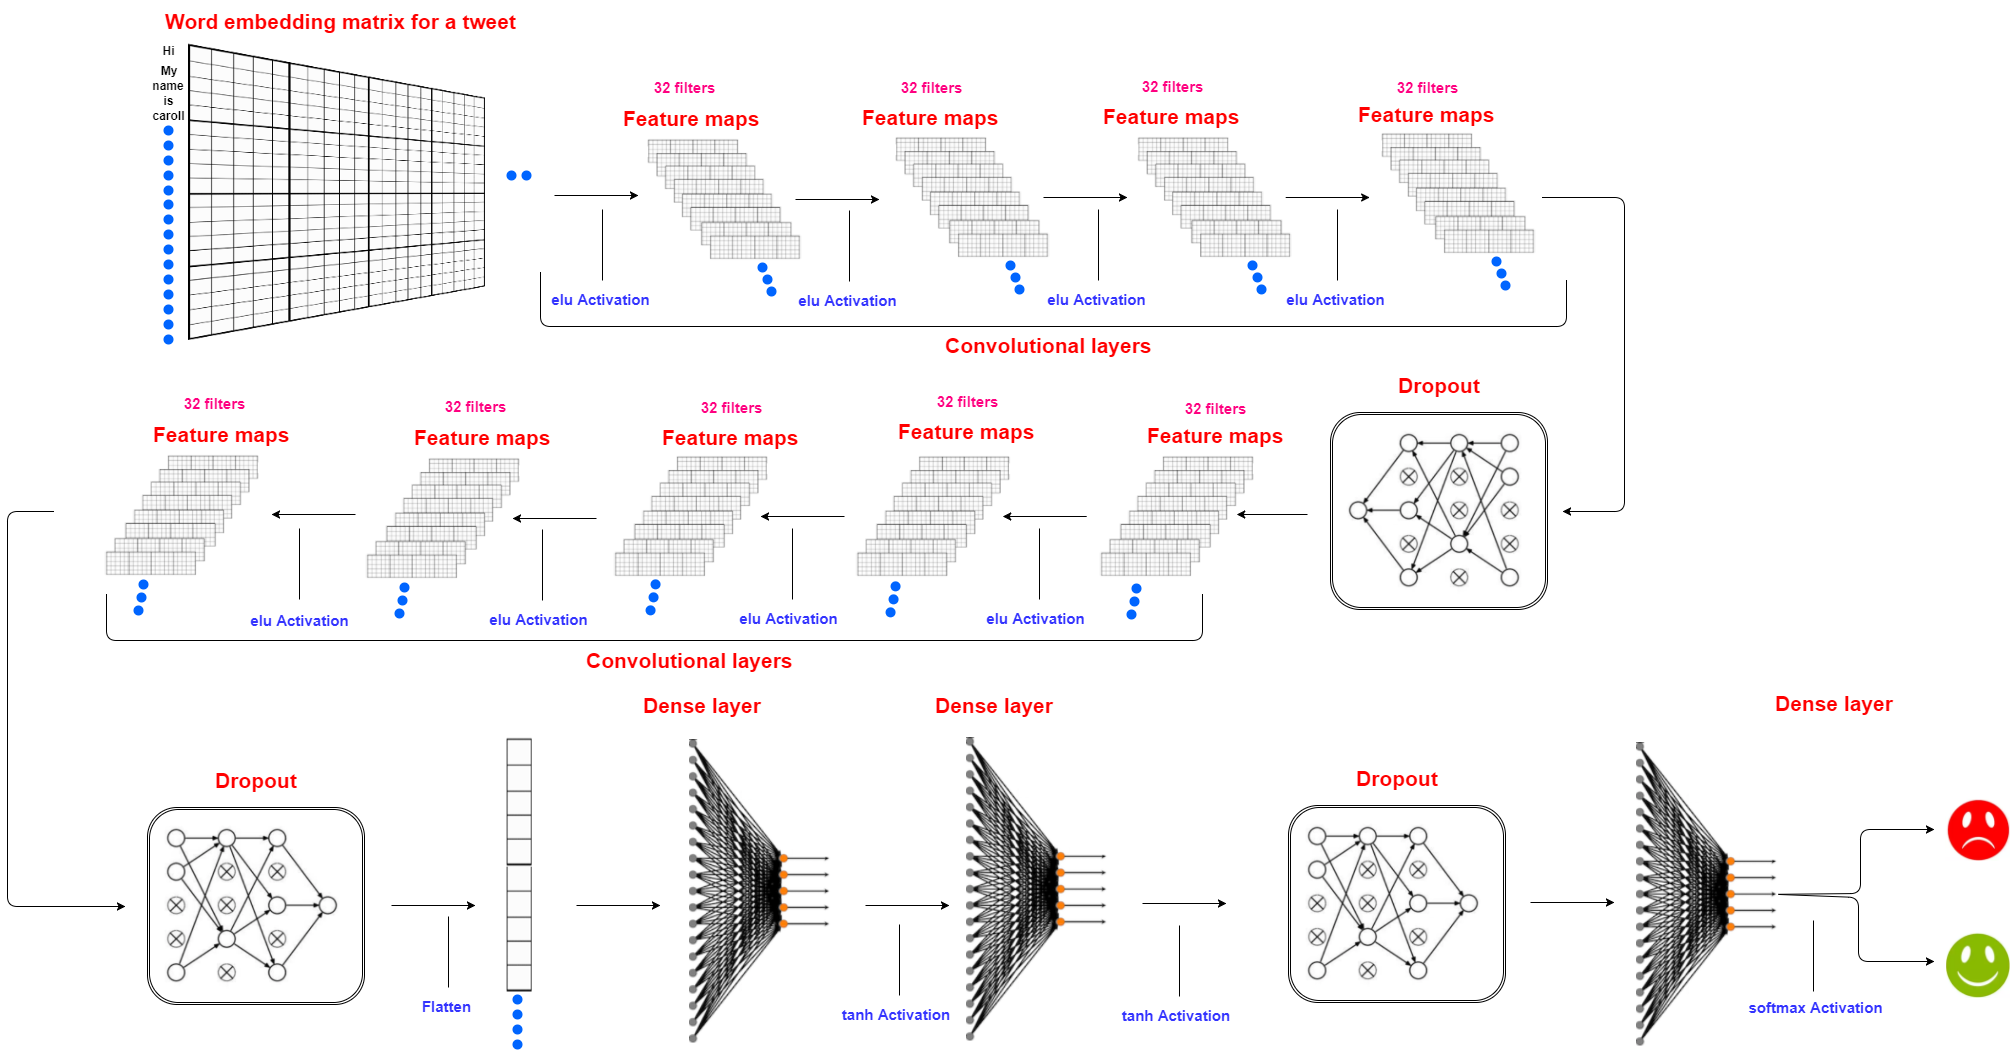
\includegraphics[width=200px]{../plots/cnn}
	\caption{Our general structure of convolutional neural network}
	\label{fig:data}
\end{figure}

Fig.6 shows the general structure of our model. We simply concatenate convolutional layers in sequential fashion. Note that we used 1D convolutional layers because our words are represented as a vector form. We did not use any pooling layer between convolutional layers because it is not fundamental to reduce dimension in this context. We also applied dropout layers before output layer as usual and between convolutional layers \cite{cnn5}in order to prevent overfitting. For hidden layers, elu is used, for first two elements of output layer tanh activation function is used and for the last element of output layer, softmax activation function is used in favor of common practice \cite{cnn6}.
Note that, the number of filters for convolutional layers, the size of the filters, activation function types regarding the type of the layer, dropout amount and the number of convolutional layers are just a subset of complete hyper parameters of this model that can be regulated in order to search optimum model.

\section{Results}
\begin{table}[ht]
	\centering
	\tiny
	\begin{tabular}{|c | c |  c | c | c |} 
		\hline
		Model & Dataset & Train acc. & Val. acc. & L2 \\
		\hline
		GloVe RNN & 0 & 0 & 0 &   \\ 
		\hline
		GloVe CNN & 0 & 0 & 0 &  \\
		\hline
		GloVe FC & 0 & 0 & 0 & \\
		\hline
		WC LR & Partial & 0.86 & 0.81 & 1000, not tuned\\
		\hline
		WC LR & Full & 0.86 & 0.83 & 1000, not tuned\\
		\hline
		WC FC 100x50 & Full & 0.86 & 0.83 & 1000, not tuned\\
		\hline
		WC FC 100x50 & Full, clean & 0 & 0 & 1\\ [1ex] 
		\hline
	\end{tabular}
	\caption{Comparison of different methods (WC=Word Count, GloVe~-- pretrained GloVe vectors, LR~-- Logistic Regression)}
	\label{tab:results}
\end{table}

The following models were considered: CNN, RNN, Logistic Regression, Fully Connected Neural Network. The best model demonstrated This (does not) correspond to already conducted experiments [99, 98, 97]. Our contribution consists of running {\em method} with {\em xxx} modified with {\em yyy} and this does (not) give an improvement of 0.01231\%
\section{Discussion}
Our experiments lack {\em zzz}, which can be improved by doing also {\em ttt}
\section{Summary}
We have shown that it is possible to predict tweets using {\em aba} better than state-of-the-art.



\begin{thebibliography}{99}

	\bibitem{twitter} \href{http://twitter.com}{Twitter}
	\bibitem{sota1} Go, Alec, Lei Huang, and Richa Bhayani. "Twitter sentiment analysis." Entropy 17 (2009): 252.
	\bibitem{sota2} Kouloumpis, Efthymios, Theresa Wilson, and Johanna D. Moore. "Twitter sentiment analysis: The good the bad and the omg!." Icwsm 11.538-541 (2011): 164.
	\bibitem{sota3} Tapan Sahni, Chinmay Chandak, Naveen Reddy, Manish Singh. "Efficient Twitter Sentiment Classification using Subjective Distant Supervision"
	\bibitem{sota4} Alec Go, Richa Bhayani,	Lei Huang. "Twitter Sentiment Classification using Distant Supervision"
	\bibitem{glove} Jeffrey Pennington, Richard Socher, Christopher D. Manning. "GloVe: Global Vectors for Word Representation"
	\bibitem{cnn1}  Kim, Y. (2014). "Convolutional neural networks for sentence classification." arXiv preprint arXiv:1408.5882.
	\bibitem{cnn2} Springenberg, J. T., Dosovitskiy, A., Brox, T., and Riedmiller, M. (2014). "Striving for simplicity: The all convolutional net." arXiv preprint arXiv 1412.6806.
	\bibitem{cnn3} Collobert, R., Weston, J., Bottou, L., Karlen, M., Kavukcuoglu, K., and Kuksa, P. (2011). Natural language processing (almost) from scratch. Journal of Machine Learning Research, 12(Aug), 2493-2537.
	\bibitem{cnn4} http://cs231n.github.io/convolutional-networks/{\#}norm
	\bibitem{cnn5} Park, S., and Kwak, N. (2016, November). "Analysis on the Dropout Effect in Convolutional Neural Networks." In Asian Conference on Computer Vision (pp. 189-204). Springer, Cham.
	\bibitem{cnn6} http://cs231n.github.io/neural-networks-1/{\#}actfun
\end{thebibliography}
\end{document}
